\documentclass{beamer}
\usetheme{Boadilla}

% ------ Basic packages -------
%\usepackage[margin=1.2in]{geometry}	% smaller margins              
\usepackage[utf8]{inputenc}			%for æ,ø,å on mac
\usepackage{amsmath,amsfonts,amssymb,amsthm,mathtools} % for mathematics
\usepackage{hyperref}					   % Clickable links to urls, internal and external references etc.
\usepackage{fancyhdr}					  % trengs for topp- og bunntekster og sidetall
\usepackage{pdfpages}					 % for å hente in pdf
%\numberwithin{equation}{section} % sub-numbers for equations
\usepackage{cite}								% For sitater og referanser
\usepackage[square,sort]{natbib}				% For referanser i klamme-parenteser  

% ------ Figures/graphic -----
\usepackage{graphicx}						%Graphic package
\usepackage{xcolor}
\usepackage{multicol}						 % for multiple columns
\usepackage[font=small,labelfont=bf,textfont=normal, format=hang]{caption}	% Configuration of captions
\usepackage{subcaption,graphicx}
\usepackage{wrapfig}  						% Wrap text around figures	
\usepackage{float} 								% To place figures correctly
\usepackage{color}							   % muliggjør farget tekst
\usepackage{tcolorbox}					   % enables color boxes
\definecolor{light-gray}{gray}{0.95} %the shade of grey that stack exchange uses
\usepackage{multirow}						
\usepackage{bm}									% usepackage bold symbols
\usepackage{xspace}							 % trengs også for fete typer


% -------- TikZ --------
\usepackage{tikz}
\usetikzlibrary{shapes.geometric, arrows}
\usetikzlibrary{matrix,chains,positioning,decorations.pathreplacing,arrows}
\tikzstyle{startstop} = [rectangle, rounded corners, minimum width=1.8cm, minimum height=1cm,text centered, draw=black, fill=blue!40]
\tikzstyle{io} = [trapezium, trapezium left angle=80, trapezium right angle=100, minimum width=1cm, minimum height=1cm, text centered, draw=black, fill=blue!20]
\tikzstyle{process} = [rectangle, minimum width=2cm, minimum height=1cm, text centered, text width=2cm, draw=black, fill=blue!5]
\tikzstyle{decision} = [diamond, minimum width=2cm, minimum height=1cm, text centered, draw=black, fill=green!30]
\tikzstyle{arrow} = [thick,->,>=stealth]

% -------- Embedded code ----------
\usepackage{listings}
\usepackage{color}
\definecolor{dkgreen}{rgb}{0,0.6,0}
\definecolor{gray}{rgb}{0.5,0.5,0.5}
\definecolor{mauve}{rgb}{0.58,0,0.82}
\lstset{frame=tb,
	language=Matlab,
	aboveskip=3mm,
	belowskip=3mm,
	showstringspaces=false,
	columns=flexible,
	basicstyle={\small\ttfamily},
	numbers=none,
	numberstyle=\tiny\color{gray},
	keywordstyle=\color{blue},
	commentstyle=\color{dkgreen},
	stringstyle=\color{mauve},
	breaklines=true,
	breakatwhitespace=true,
	tabsize=3
}

%% Nye kommandoer/snarveier
%\newcommand{\pd}{\ensuremath{\partial}} 			 % <---------- Partial derivative
%\newcommand{\ul}{\ensuremath{\underline}} 			% <---------- underline for easier vector notation
%\newcommand{\D}{\mathrm{D}}							   % <---------- Material derivate
%\newcommand{\vb}{\bm {v}\xspace}						% <---------- bold,italic v
%\newcommand{\wb}{\bm {w}\xspace}					  % <---------- bold,italic w
\newcommand{\ub}{\bm {u}\xspace}						% <---------- bold,italic u					
%\newcommand{\gb}{\bm {g}\xspace}					   % <---------- bold,italic g
%\newcommand{\rb}{\bm {r}\xspace}						 % <---------- bold,italic r
%\newcommand{\fb}{\bm {f}\xspace}						 % <---------- bold,italic f
%\newcommand{\Fb}{\bm {F}\xspace}						% <---------- bold,italic f
%\newcommand{\ib}{\bm {i}\xspace}						  % <---------- bold,italic i
%\newcommand{\jb}{\bm {j}\xspace}						  % <---------- bold,italic j
%\newcommand{\yb}{\bm {y}\xspace}						% <---------- bold,italic y
%\newcommand{\xb}{\bm {x}\xspace}						% <---------- bold,italic x
%\newcommand{\taub}{\bm {\tau}\xspace}				 % <---------- bold,italic tau
%\newcommand{\lambdb}{\bm {\lambda}\xspace}
%\newcommand{\til}{\ensuremath{\widetilde}} 		% <---------- tilde
%\newcommand{\mub}{\bm {\mu}\xspace}				% <---------- bold, italic mu	
%\newcommand{\h}{\ensuremath{\hat}} 					% <---------- hat
%\newcommand{\dr}{\mathrm{d}}								% <---------- derivate
% \renewcommand{\thefootnote}{\roman{footnote}}	% Fotnoter med romerske symboler istedenfor tall



% Første side 
\title{Introduction to WRF}
\subtitle{Model framework}
\author{Torgeir Blæsterdalen}
\institute{Department of Industrial Engineering, UiT-The Arctic University of Norway}
\date{\today}



% ------ Utseende og forside -----
\begin{document}
\begin{frame}
\titlepage
\end{frame}

\begin{frame}{Lecture topics}
\begin{enumerate}
	\item WRF components and its workflow
	\item Domain configurations and nesting
	\item Vertical resolution and $\eta$-levels
	\item Temporal resolution and the time step contraint
\end{enumerate}
\end{frame}


\begin{frame}{1. WRF components and its workflow}

\begin{center}
	\resizebox{\textwidth}{!}{%
	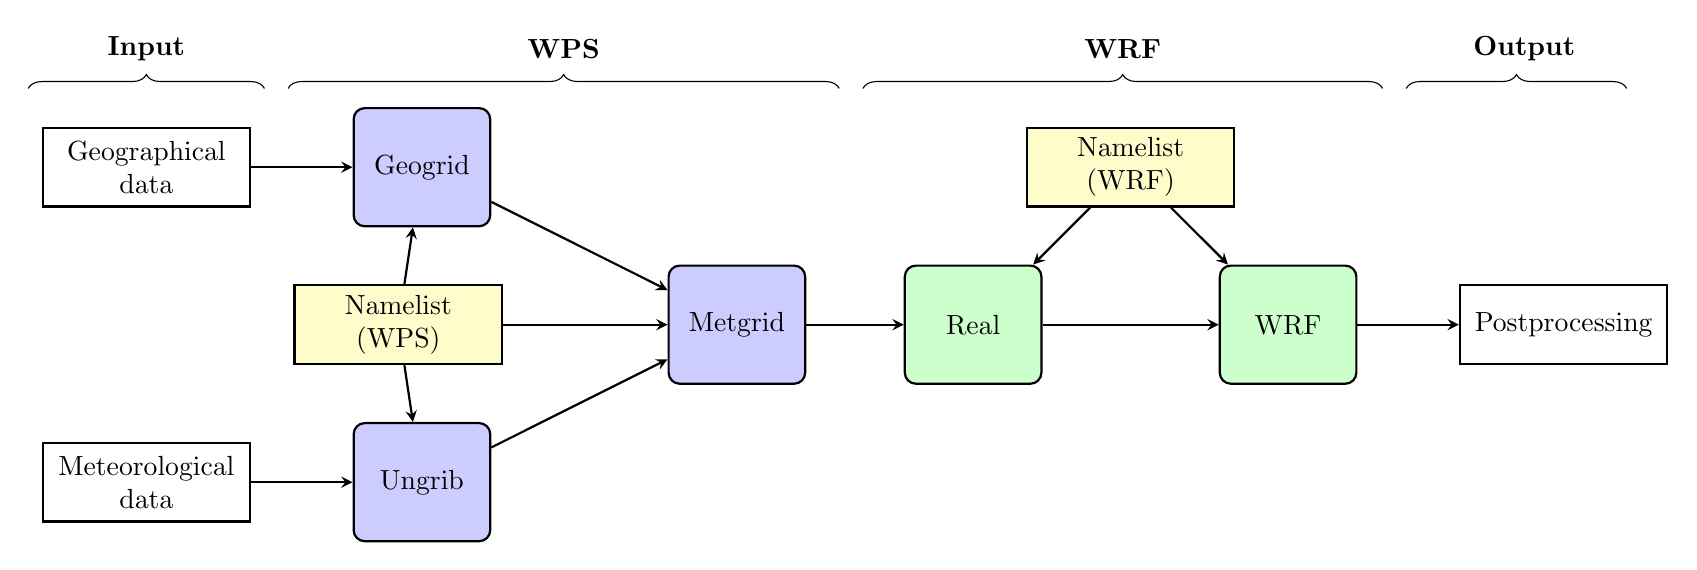
\begin{tikzpicture}
	\coordinate (geogdata) at (-1,7);
	\coordinate (metgrib) at (-1,3);
	\coordinate (namelist1) at (2.2,5); 
	\coordinate (geogrid) at (2.5,7);
	\coordinate (ungrib) at (2.5,3);
	\coordinate (metgrid) at (6.5,5);
	\coordinate (namelist2) at (11.5,7);
	\coordinate (real) at (9.5,5);
	\coordinate (wrf) at (13.5,5);
	\coordinate (postpro) at (17,5);
	\tikzstyle{arrow} = [thick, ->, >=stealth]
	% Input to WPS (and postprocessing)
	\begin{scope}[every node/.style={draw, thick, rectangle, text width=2.4cm, minimum height=1cm, text centered}]
	\node[name=geogdata] at (geogdata) {Geographical data};
	\node[name=metgrib] at (metgrib) {Meteorological data};
	\node[name=postpro] at (postpro) {Postprocessing};
	\end{scope}
	% Namelists
	\begin{scope}[every node/.style={draw, thick, fill=yellow!20, rectangle, text width=2.4cm, minimum height=1cm, text centered}]
	\node[name=namelist1] at (namelist1) {Namelist (WPS)};
	\node[name=namelist2] at (namelist2) {Namelist (WRF)};
	\end{scope}
	% WPS
	\begin{scope}[every node/.style={draw, thick, fill=blue!20, rectangle, rounded corners, text width=1.5cm, minimum height=1.5cm, text centered}]
	\node[name=geogrid] at (geogrid) { Geogrid};
	\node[name=ungrib] at (ungrib) {Ungrib};
	\node[name=metgrid] at (metgrid) {Metgrid};
	\end{scope}
	% WRF
	\begin{scope}[every node/.style={draw, thick, fill=green!20, rectangle, rounded corners, text width=1.5cm, minimum height=1.5cm, text centered}]
	\node[name=real] at (real) {Real};
	\node[name=wrf] at (wrf) {WRF};
	\end{scope}
	\draw [arrow] (geogdata)--(geogrid);
	\draw [arrow] (namelist1)--(geogrid);
	\draw [arrow] (geogrid)--(metgrid);
	\draw [arrow] (namelist1)--(ungrib);
	\draw [arrow] (namelist1)--(metgrid);
	\draw [arrow] (metgrib)--(ungrib);
	\draw [arrow] (ungrib)--(metgrid);
	\draw [arrow] (metgrid)--(real);
	\draw [arrow] (namelist2)--(real);
	\draw [arrow] (namelist2)--(wrf);
	\draw [arrow] (real)--(wrf);
	\draw [arrow] (wrf)--(postpro);
	% curly braces
	\draw[decorate,decoration={brace,amplitude=5pt}] (-2.5,8) -- (0.5,8);  	
	\draw[decorate,decoration={brace,amplitude=5pt}] (0.8,8) -- (7.8,8);
	\draw[decorate,decoration={brace,amplitude=5pt}] (8.1,8) -- (14.7,8);
	\draw[decorate,decoration={brace,amplitude=5pt}] (15,8) -- (17.8,8);		
	% Nodes
	\draw (-1, 8.5) node{\bfseries Input};
	\draw (4.3, 8.5) node{\bfseries WPS};
	\draw (11.4, 8.5) node{\bfseries WRF};
	\draw (16.5, 8.5) node{\bfseries Output};
\end{tikzpicture}
}%
\end{center}
\end{frame}


\begin{frame}
\begin{center}
	\resizebox{\textwidth}{!}{%
		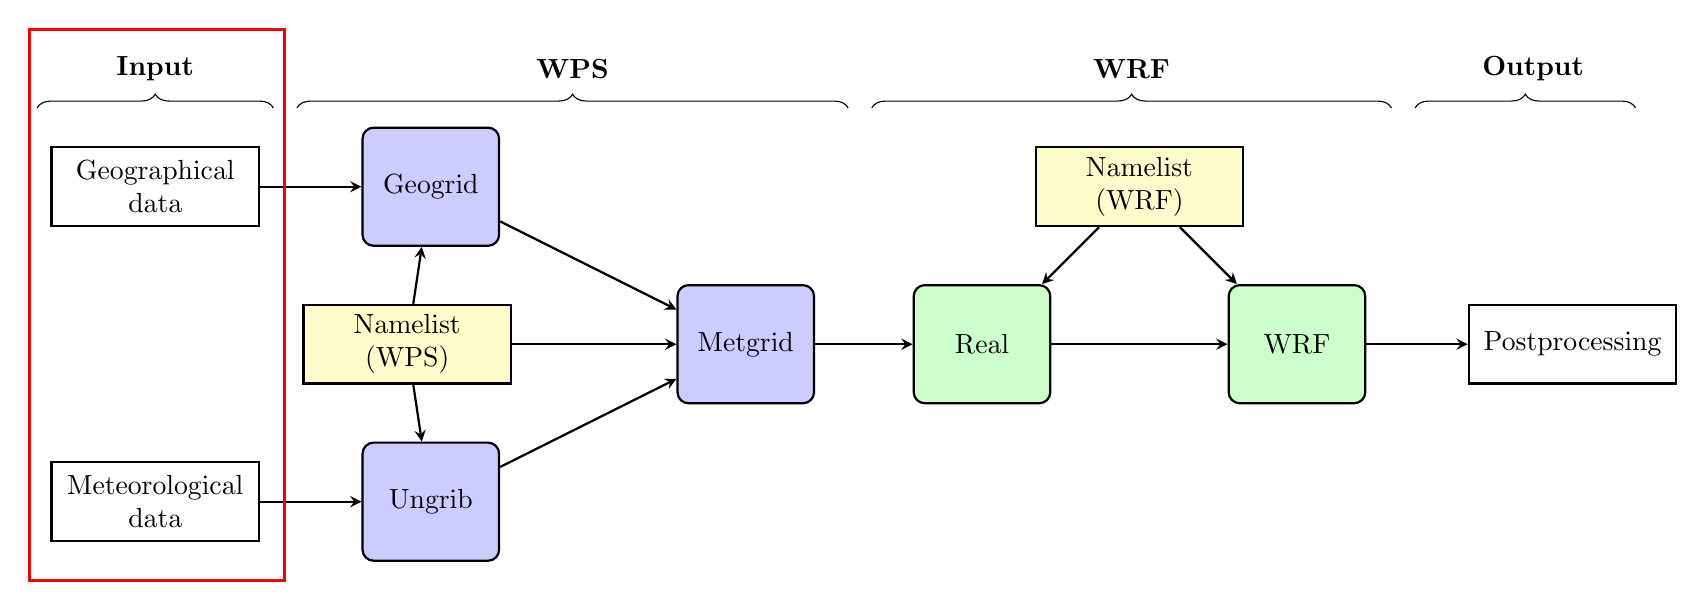
\begin{tikzpicture}
		\coordinate (geogdata) at (-1,7);
		\coordinate (metgrib) at (-1,3);
		\coordinate (namelist1) at (2.2,5); 
		\coordinate (geogrid) at (2.5,7);
		\coordinate (ungrib) at (2.5,3);
		\coordinate (metgrid) at (6.5,5);
		\coordinate (namelist2) at (11.5,7);
		\coordinate (real) at (9.5,5);
		\coordinate (wrf) at (13.5,5);
		\coordinate (postpro) at (17,5);
		\tikzstyle{arrow} = [thick, ->, >=stealth]
		% Input to WPS (and postprocessing)
		\begin{scope}[every node/.style={draw, thick, rectangle, text width=2.4cm, minimum height=1cm, text centered}]
		\node[name=geogdata] at (geogdata) {Geographical data};
		\node[name=metgrib] at (metgrib) {Meteorological data};
		\node[name=postpro] at (postpro) {Postprocessing};
		\end{scope}
		% Namelists
		\begin{scope}[every node/.style={draw, thick, fill=yellow!20, rectangle, text width=2.4cm, minimum height=1cm, text centered}]
		\node[name=namelist1] at (namelist1) {Namelist (WPS)};
		\node[name=namelist2] at (namelist2) {Namelist (WRF)};
		\end{scope}
		% WPS
		\begin{scope}[every node/.style={draw, thick, fill=blue!20, rectangle, rounded corners, text width=1.5cm, minimum height=1.5cm, text centered}]
		\node[name=geogrid] at (geogrid) { Geogrid};
		\node[name=ungrib] at (ungrib) {Ungrib};
		\node[name=metgrid] at (metgrid) {Metgrid};
		\end{scope}
		% WRF
		\begin{scope}[every node/.style={draw, thick, fill=green!20, rectangle, rounded corners, text width=1.5cm, minimum height=1.5cm, text centered}]
		\node[name=real] at (real) {Real};
		\node[name=wrf] at (wrf) {WRF};
		\end{scope}
		\draw [arrow] (geogdata)--(geogrid);
		\draw [arrow] (namelist1)--(geogrid);
		\draw [arrow] (geogrid)--(metgrid);
		\draw [arrow] (namelist1)--(ungrib);
		\draw [arrow] (namelist1)--(metgrid);
		\draw [arrow] (metgrib)--(ungrib);
		\draw [arrow] (ungrib)--(metgrid);
		\draw [arrow] (metgrid)--(real);
		\draw [arrow] (namelist2)--(real);
		\draw [arrow] (namelist2)--(wrf);
		\draw [arrow] (real)--(wrf);
		\draw [arrow] (wrf)--(postpro);
		% curly braces
		\draw[decorate,decoration={brace,amplitude=5pt}] (-2.5,8) -- (0.5,8);  	
		\draw[decorate,decoration={brace,amplitude=5pt}] (0.8,8) -- (7.8,8);
		\draw[decorate,decoration={brace,amplitude=5pt}] (8.1,8) -- (14.7,8);
		\draw[decorate,decoration={brace,amplitude=5pt}] (15,8) -- (17.8,8);		
		% Nodes
		\draw (-1, 8.5) node{\bfseries Input};
		\draw (4.3, 8.5) node{\bfseries WPS};
		\draw (11.4, 8.5) node{\bfseries WRF};
		\draw (16.5, 8.5) node{\bfseries Output};
		% Red rectangle around Input
		\draw[red, line width=0.4mm] (-2.6,2) rectangle(0.64,9);
		\end{tikzpicture}
	}%
\end{center}
Input to preprocessing:
\begin{itemize}
	\item Geographical data: topography, type of vegetation, albedo, lake depths, soil types 
	\item Meteorological boundary conditions: pressure and surface variables, e.g. Cloud cover, potential vorticity, humidity, temperature, wind direction and magnitude, etc.
\end{itemize}
\end{frame}




\begin{frame}
\begin{center}
	\resizebox{\textwidth}{!}{%
		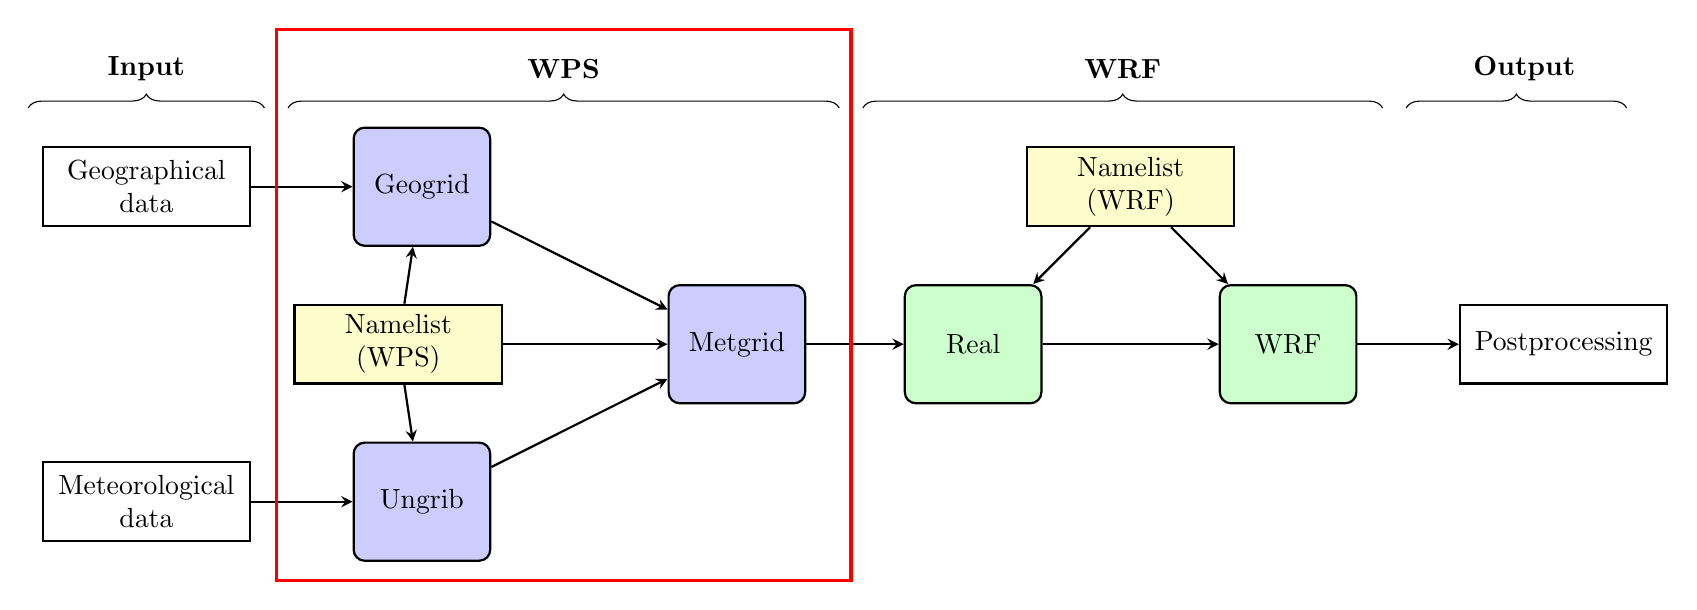
\begin{tikzpicture}
		\coordinate (geogdata) at (-1,7);
		\coordinate (metgrib) at (-1,3);
		\coordinate (namelist1) at (2.2,5); 
		\coordinate (geogrid) at (2.5,7);
		\coordinate (ungrib) at (2.5,3);
		\coordinate (metgrid) at (6.5,5);
		\coordinate (namelist2) at (11.5,7);
		\coordinate (real) at (9.5,5);
		\coordinate (wrf) at (13.5,5);
		\coordinate (postpro) at (17,5);
		\tikzstyle{arrow} = [thick, ->, >=stealth]
		% Input to WPS (and postprocessing)
		\begin{scope}[every node/.style={draw, thick, rectangle, text width=2.4cm, minimum height=1cm, text centered}]
		\node[name=geogdata] at (geogdata) {Geographical data};
		\node[name=metgrib] at (metgrib) {Meteorological data};
		\node[name=postpro] at (postpro) {Postprocessing};
		\end{scope}
		% Namelists
		\begin{scope}[every node/.style={draw, thick, fill=yellow!20, rectangle, text width=2.4cm, minimum height=1cm, text centered}]
		\node[name=namelist1] at (namelist1) {Namelist (WPS)};
		\node[name=namelist2] at (namelist2) {Namelist (WRF)};
		\end{scope}
		% WPS
		\begin{scope}[every node/.style={draw, thick, fill=blue!20, rectangle, rounded corners, text width=1.5cm, minimum height=1.5cm, text centered}]
		\node[name=geogrid] at (geogrid) { Geogrid};
		\node[name=ungrib] at (ungrib) {Ungrib};
		\node[name=metgrid] at (metgrid) {Metgrid};
		\end{scope}
		% WRF
		\begin{scope}[every node/.style={draw, thick, fill=green!20, rectangle, rounded corners, text width=1.5cm, minimum height=1.5cm, text centered}]
		\node[name=real] at (real) {Real};
		\node[name=wrf] at (wrf) {WRF};
		\end{scope}
		\draw [arrow] (geogdata)--(geogrid);
		\draw [arrow] (namelist1)--(geogrid);
		\draw [arrow] (geogrid)--(metgrid);
		\draw [arrow] (namelist1)--(ungrib);
		\draw [arrow] (namelist1)--(metgrid);
		\draw [arrow] (metgrib)--(ungrib);
		\draw [arrow] (ungrib)--(metgrid);
		\draw [arrow] (metgrid)--(real);
		\draw [arrow] (namelist2)--(real);
		\draw [arrow] (namelist2)--(wrf);
		\draw [arrow] (real)--(wrf);
		\draw [arrow] (wrf)--(postpro);
		% curly braces
		\draw[decorate,decoration={brace,amplitude=5pt}] (-2.5,8) -- (0.5,8);  	
		\draw[decorate,decoration={brace,amplitude=5pt}] (0.8,8) -- (7.8,8);
		\draw[decorate,decoration={brace,amplitude=5pt}] (8.1,8) -- (14.7,8);
		\draw[decorate,decoration={brace,amplitude=5pt}] (15,8) -- (17.8,8);		
		% Nodes
		\draw (-1, 8.5) node{\bfseries Input};
		\draw (4.3, 8.5) node{\bfseries WPS};
		\draw (11.4, 8.5) node{\bfseries WRF};
		\draw (16.5, 8.5) node{\bfseries Output};
		% Red rectangle around WPS
		\draw[red, line width=0.4mm] (.65,2) rectangle(7.95,9);
		\end{tikzpicture}
	}%
\end{center}
WRF preprocessing system (WPS):
\begin{itemize}
	\item Namelist (WPS): Controls the WPS framework like core, simulation time, domains and input data.
	\item Geogrid: Interpolating the terrestrial input data.
	\item Ungrib: Unpacking and the meteorological input data and makes them readable.
	\item Metgrid: Horizontally interpolating the meteorological data onto the simulation domain.
\end{itemize}
\end{frame}



\begin{frame}
\begin{center}
	\resizebox{\textwidth}{!}{%
		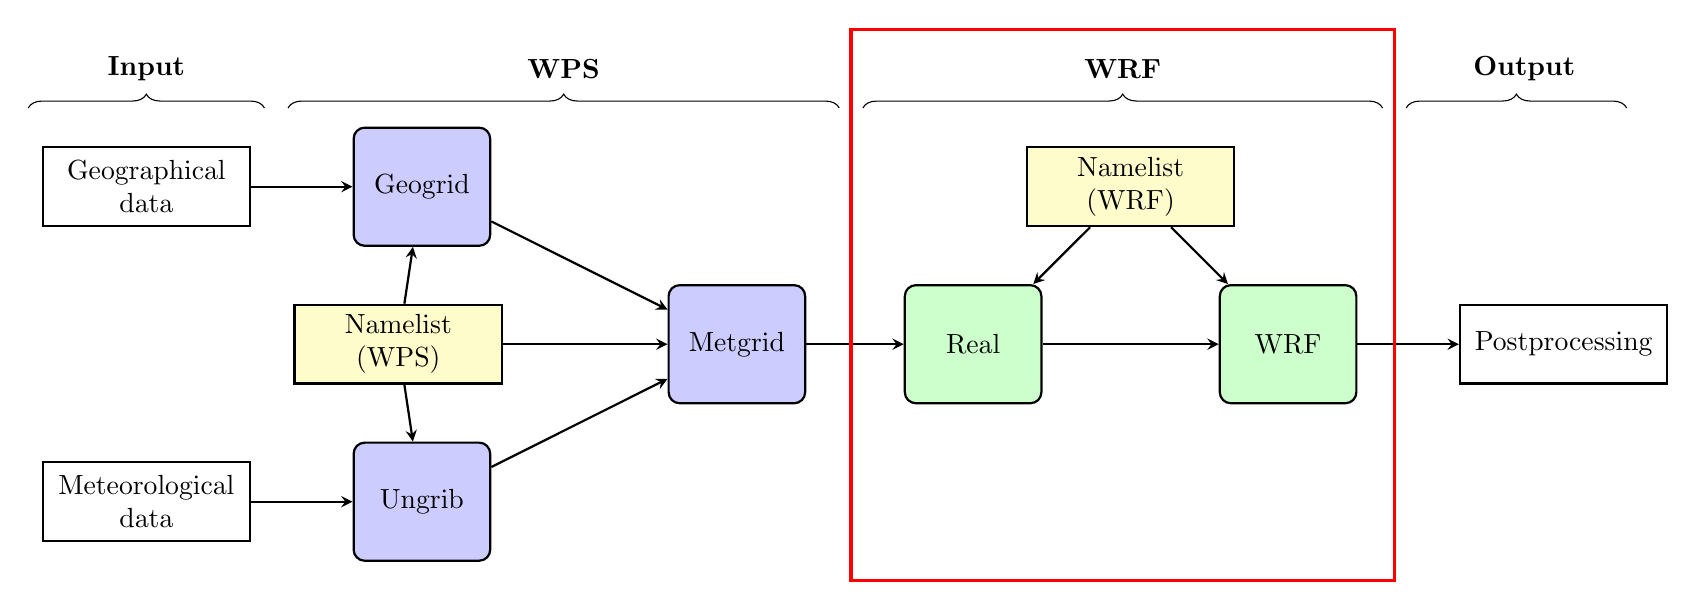
\begin{tikzpicture}
		\coordinate (geogdata) at (-1,7);
		\coordinate (metgrib) at (-1,3);
		\coordinate (namelist1) at (2.2,5); 
		\coordinate (geogrid) at (2.5,7);
		\coordinate (ungrib) at (2.5,3);
		\coordinate (metgrid) at (6.5,5);
		\coordinate (namelist2) at (11.5,7);
		\coordinate (real) at (9.5,5);
		\coordinate (wrf) at (13.5,5);
		\coordinate (postpro) at (17,5);
		\tikzstyle{arrow} = [thick, ->, >=stealth]
		% Input to WPS (and postprocessing)
		\begin{scope}[every node/.style={draw, thick, rectangle, text width=2.4cm, minimum height=1cm, text centered}]
		\node[name=geogdata] at (geogdata) {Geographical data};
		\node[name=metgrib] at (metgrib) {Meteorological data};
		\node[name=postpro] at (postpro) {Postprocessing};
		\end{scope}
		% Namelists
		\begin{scope}[every node/.style={draw, thick, fill=yellow!20, rectangle, text width=2.4cm, minimum height=1cm, text centered}]
		\node[name=namelist1] at (namelist1) {Namelist (WPS)};
		\node[name=namelist2] at (namelist2) {Namelist (WRF)};
		\end{scope}
		% WPS
		\begin{scope}[every node/.style={draw, thick, fill=blue!20, rectangle, rounded corners, text width=1.5cm, minimum height=1.5cm, text centered}]
		\node[name=geogrid] at (geogrid) { Geogrid};
		\node[name=ungrib] at (ungrib) {Ungrib};
		\node[name=metgrid] at (metgrid) {Metgrid};
		\end{scope}
		% WRF
		\begin{scope}[every node/.style={draw, thick, fill=green!20, rectangle, rounded corners, text width=1.5cm, minimum height=1.5cm, text centered}]
		\node[name=real] at (real) {Real};
		\node[name=wrf] at (wrf) {WRF};
		\end{scope}
		\draw [arrow] (geogdata)--(geogrid);
		\draw [arrow] (namelist1)--(geogrid);
		\draw [arrow] (geogrid)--(metgrid);
		\draw [arrow] (namelist1)--(ungrib);
		\draw [arrow] (namelist1)--(metgrid);
		\draw [arrow] (metgrib)--(ungrib);
		\draw [arrow] (ungrib)--(metgrid);
		\draw [arrow] (metgrid)--(real);
		\draw [arrow] (namelist2)--(real);
		\draw [arrow] (namelist2)--(wrf);
		\draw [arrow] (real)--(wrf);
		\draw [arrow] (wrf)--(postpro);
		% curly braces
		\draw[decorate,decoration={brace,amplitude=5pt}] (-2.5,8) -- (0.5,8);  	
		\draw[decorate,decoration={brace,amplitude=5pt}] (0.8,8) -- (7.8,8);
		\draw[decorate,decoration={brace,amplitude=5pt}] (8.1,8) -- (14.7,8);
		\draw[decorate,decoration={brace,amplitude=5pt}] (15,8) -- (17.8,8);		
		% Nodes
		\draw (-1, 8.5) node{\bfseries Input};
		\draw (4.3, 8.5) node{\bfseries WPS};
		\draw (11.4, 8.5) node{\bfseries WRF};
		\draw (16.5, 8.5) node{\bfseries Output};
		% Red rectangle around WRF
		\draw[red, line width=0.4mm] (7.95,2) rectangle(14.85,9);
		\end{tikzpicture}
	}%
\end{center}

\begin{itemize}
	\item Namelist (WRF): Defining all the simulation parameters. All parameters and physical options are specified in this script.
	\item Real: Vertically interpolates the meteorological fields to the model grid. The output of \texttt{Real.exe} is fully interpolated 4-dimensional simulation data.
	\item WRF: The 4-D interpolated boundary values is simulated using WRF's dynamical solver.   
\end{itemize}
\end{frame}



\begin{frame}
\begin{center}
	\resizebox{\textwidth}{!}{%
		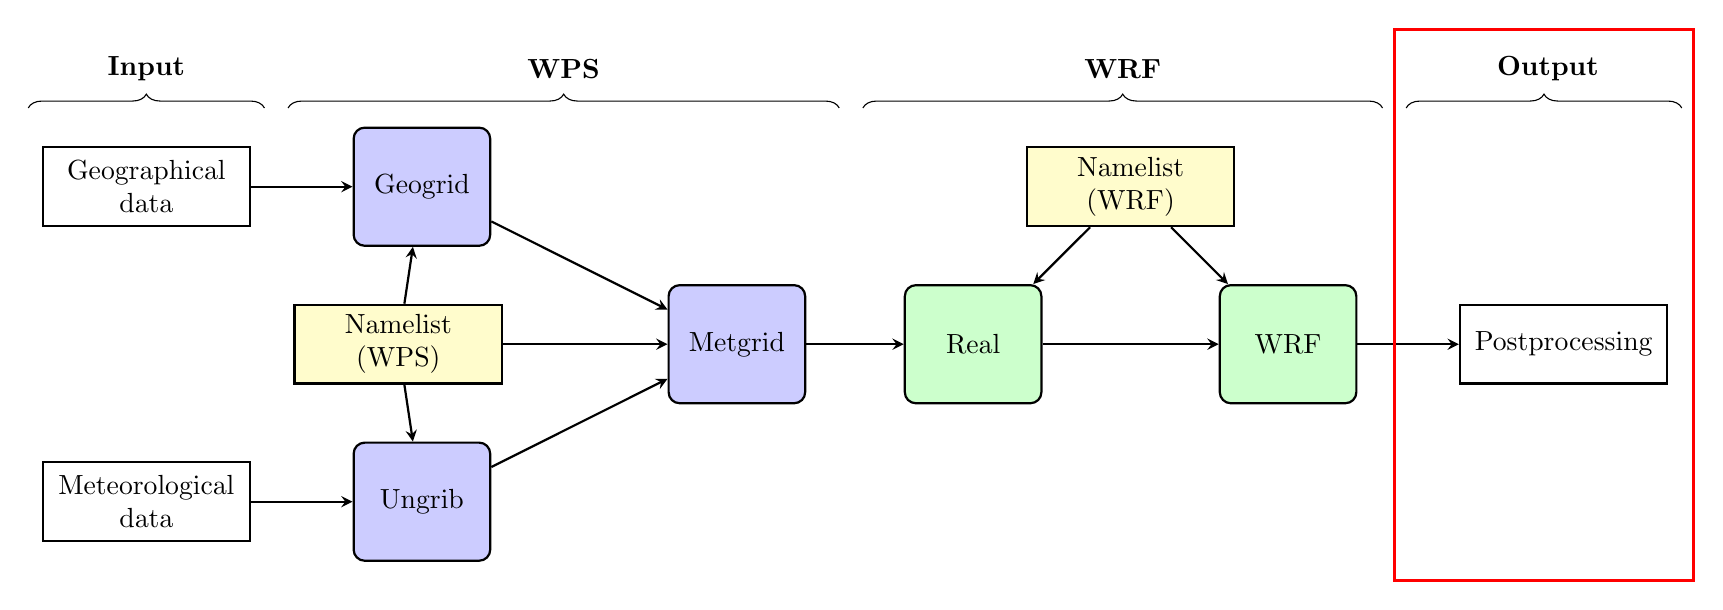
\begin{tikzpicture}
		\coordinate (geogdata) at (-1,7);
		\coordinate (metgrib) at (-1,3);
		\coordinate (namelist1) at (2.2,5); 
		\coordinate (geogrid) at (2.5,7);
		\coordinate (ungrib) at (2.5,3);
		\coordinate (metgrid) at (6.5,5);
		\coordinate (namelist2) at (11.5,7);
		\coordinate (real) at (9.5,5);
		\coordinate (wrf) at (13.5,5);
		\coordinate (postpro) at (17,5);
		\tikzstyle{arrow} = [thick, ->, >=stealth]
		% Input to WPS (and postprocessing)
		\begin{scope}[every node/.style={draw, thick, rectangle, text width=2.4cm, minimum height=1cm, text centered}]
		\node[name=geogdata] at (geogdata) {Geographical data};
		\node[name=metgrib] at (metgrib) {Meteorological data};
		\node[name=postpro] at (postpro) {Postprocessing};
		\end{scope}
		% Namelists
		\begin{scope}[every node/.style={draw, thick, fill=yellow!20, rectangle, text width=2.4cm, minimum height=1cm, text centered}]
		\node[name=namelist1] at (namelist1) {Namelist (WPS)};
		\node[name=namelist2] at (namelist2) {Namelist (WRF)};
		\end{scope}
		% WPS
		\begin{scope}[every node/.style={draw, thick, fill=blue!20, rectangle, rounded corners, text width=1.5cm, minimum height=1.5cm, text centered}]
		\node[name=geogrid] at (geogrid) { Geogrid};
		\node[name=ungrib] at (ungrib) {Ungrib};
		\node[name=metgrid] at (metgrid) {Metgrid};
		\end{scope}
		% WRF
		\begin{scope}[every node/.style={draw, thick, fill=green!20, rectangle, rounded corners, text width=1.5cm, minimum height=1.5cm, text centered}]
		\node[name=real] at (real) {Real};
		\node[name=wrf] at (wrf) {WRF};
		\end{scope}
		\draw [arrow] (geogdata)--(geogrid);
		\draw [arrow] (namelist1)--(geogrid);
		\draw [arrow] (geogrid)--(metgrid);
		\draw [arrow] (namelist1)--(ungrib);
		\draw [arrow] (namelist1)--(metgrid);
		\draw [arrow] (metgrib)--(ungrib);
		\draw [arrow] (ungrib)--(metgrid);
		\draw [arrow] (metgrid)--(real);
		\draw [arrow] (namelist2)--(real);
		\draw [arrow] (namelist2)--(wrf);
		\draw [arrow] (real)--(wrf);
		\draw [arrow] (wrf)--(postpro);
		% curly braces
		\draw[decorate,decoration={brace,amplitude=5pt}] (-2.5,8) -- (0.5,8);  	
		\draw[decorate,decoration={brace,amplitude=5pt}] (0.8,8) -- (7.8,8);
		\draw[decorate,decoration={brace,amplitude=5pt}] (8.1,8) -- (14.7,8);
		\draw[decorate,decoration={brace,amplitude=5pt}] (15,8) -- (18.5,8);		
		% Nodes
		\draw (-1, 8.5) node{\bfseries Input};
		\draw (4.3, 8.5) node{\bfseries WPS};
		\draw (11.4, 8.5) node{\bfseries WRF};
		\draw (16.8, 8.5) node{\bfseries Output};
		% Red rectangle around WRF
		\draw[red, line width=0.4mm] (14.85,2) rectangle(18.65,9);
		\end{tikzpicture}
	}%
\end{center}
Postprocessing:\\
The output of the WRF model is NetCDF files containing more than 150 variables. 
\end{frame}


\begin{frame}
\begin{figure}[htp]
	\centering
	\begin{subfigure}{0.49\textwidth} 
		\centering
		\includegraphics[width=.8\textwidth]{../../Figures/60mWindField_10dec_v2}
	\end{subfigure}
	\begin{subfigure}{0.49\textwidth}
		\centering
		\includegraphics[width=.8\textwidth]{../../Figures/TKE_WindBarbs_10dec_v2}
	\end{subfigure}
	\centering
	\begin{subfigure}{0.49\textwidth} 
		\centering
		\includegraphics[width=.8\textwidth]{../../Figures/SnowDepth_10mar}
	\end{subfigure}
	\begin{subfigure}{0.49\textwidth}
		\centering
		\includegraphics[width=.8\textwidth]{../../Figures/CloudCover_10mar_eta13}
	\end{subfigure}
\end{figure}
\end{frame}




\begin{frame}{2. Domain configurations and nesting}
\begin{figure}[htp]
	\centering
	\begin{subfigure}{0.49\textwidth} 
		\centering
		\includegraphics[width=\textwidth]{../../Figures/domains_Rieppi}
	\end{subfigure}
	\begin{subfigure}{0.48\textwidth}
		\centering
		\resizebox{\linewidth}{!}{
			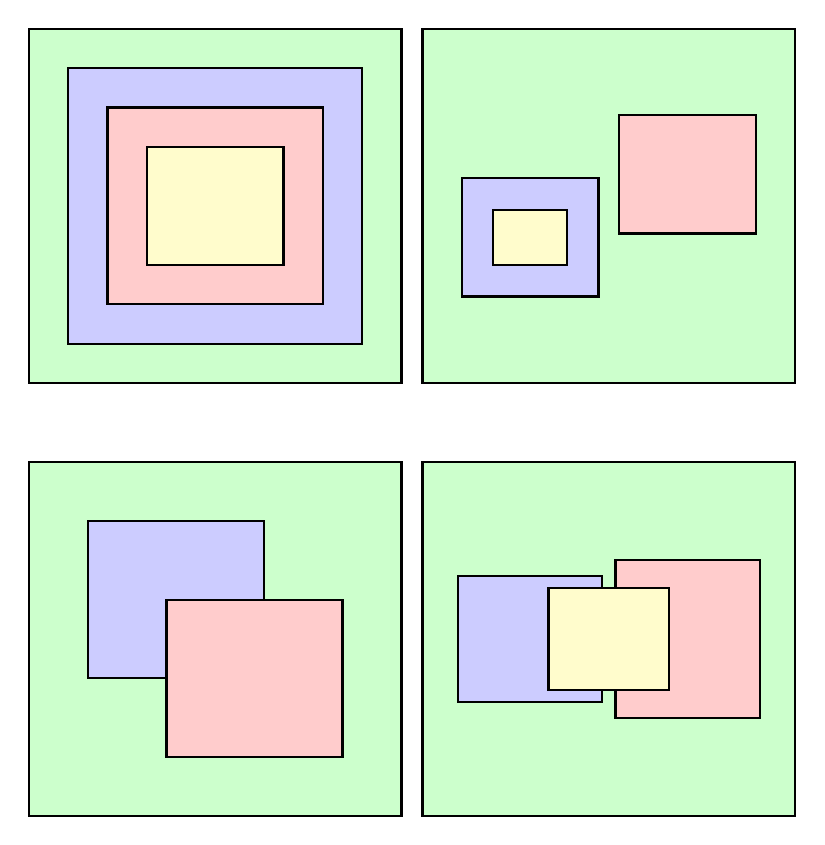
\begin{tikzpicture}
			% a
			\coordinate (D011) at (1,8.5);
			\coordinate (D021) at (1,8.5);
			\coordinate (D031) at (1,8.5);
			\coordinate (D041) at (1,8.5);
			% b
			\coordinate (D012) at (6,8.5);
			\coordinate (D022) at (5,8.1);
			\coordinate (D032) at (7,8.9);
			\coordinate (D042) at (5,8.1);
			% c
			\coordinate (D013) at (1,3);
			\coordinate (D023) at (0.5,3.5);
			\coordinate (D033) at (1.5,2.5);
			% d
			\coordinate (D014) at (6,3);
			\coordinate (D024) at (5,3);
			\coordinate (D034) at (7,3);
			\coordinate (D044) at (6,3);
			\begin{scope}[every node/.style={draw, thick, fill=green!20, rectangle, text width=4.5cm, minimum height=4.5cm, text centered}]
			\node[name=D011] at (D011) {};
			\node[name=D012] at (D012) {};
			\node[name=D013] at (D013) {};
			\node[name=D014] at (D014) {};
			\end{scope}
			\begin{scope}[every node/.style={draw, thick, fill=blue!20, rectangle, text width=3.5cm, minimum height=3.5cm, text centered}]
			\node[name=D021] at (D021) {};
			\end{scope}
			\begin{scope}[every node/.style={draw, thick, fill=blue!20, rectangle, text width=1.5cm, minimum height=1.5cm, text centered}]
			\node[name=D022] at (D022) {};
			\end{scope}
			\begin{scope}[every node/.style={draw, thick, fill=red!20, rectangle, text width=2.5cm, minimum height=2.5cm, text centered}]
			\node[name=D031] at (D031) {};
			\end{scope}
			\begin{scope}[every node/.style={draw, thick, fill=red!20, rectangle, text width=1.5cm, minimum height=1.5cm, text centered}]
			\node[name=D032] at (D032) {};
			\end{scope}
			\begin{scope}[every node/.style={draw, thick, fill=yellow!20, rectangle, text width=1.5cm, minimum height=1.5cm, text centered}]
			\node[name=D031] at (D031) {};
			\end{scope}
			\begin{scope}[every node/.style={draw, thick, fill=blue!20, rectangle, text width=2cm, minimum height=2cm, text centered}]
			\node[name=D023] at (D023) {};
			\end{scope}	
			\begin{scope}[every node/.style={draw, thick, fill=red!20, rectangle, text width=2cm, minimum height=2cm, text centered}]
			\node[name=D033] at (D033) {};
			\end{scope}
			\begin{scope}[every node/.style={draw, thick, fill=blue!20, rectangle, text width=1.6cm, minimum height=1.6cm, text centered}]
			\node[name=D024] at (D024) {};
			\end{scope}
			\begin{scope}[every node/.style={draw, thick, fill=red!20, rectangle, text width=1.6cm, minimum height=2cm, text centered}]
			\node[name=D034] at (D034) {};
			\end{scope}
			\begin{scope}[every node/.style={draw, thick, fill=yellow!20, rectangle, text width=1.3cm, minimum height=1.3cm, text centered}]
			\node[name=D044] at (D044) {};
			\end{scope}
			\begin{scope}[every node/.style={draw, thick, fill=yellow!20, rectangle, text width=0.7cm, minimum height=0.7cm, text centered}]
			\node[name=D042] at (D042) {};
			\end{scope}
			\end{tikzpicture}
		}	
	\end{subfigure}
\end{figure}
\end{frame}


\begin{frame}{3. Vertical resolution and $\eta$-levels}
\begin{multicols}{2}
The $\eta$ vertical coordinate was first defined by \cite{mesinger1984blocking}. The ground surface is the first $\eta$-coordinate. The subsequent coordinates are pressure based and normalized. The $\eta$-levels in the WRF model is given in \cite{skamarock2005description} as:
\begin{equation*}
	\eta = \frac{p_h - p_{ht}}{\mu_d},
\end{equation*}
where $\mu_d = p_{hs} - p_{ht}$. $p_h$ is hydrostatic component of  the pressure. $p_{hs}$ and $p_{ht}$ is pressure along the surface and the top boundary respectively. 
\begin{figure}[htp]
	\centering
	\centering
	\includegraphics[width=0.3\textwidth]{../../Figures/eta_levels}
\end{figure}
The figure above illustrates the height coordinates in the WRF model. Image from \citet{skamarock2008description}.
\end{multicols}
\end{frame}

\begin{frame}
\begin{figure}[htp]
	\centering
	\begin{subfigure}{0.49\textwidth} 
		\centering
		\includegraphics[width=\textwidth]{../../Figures/HeightCoordinatesWRF}
	\end{subfigure}
	\begin{subfigure}{0.49\textwidth}
		\centering
		\includegraphics[width=\textwidth]{../../Figures/HeigtCoordinatesWRF_1_10}
	\end{subfigure}
\end{figure}
\end{frame}


\begin{frame}[fragile,allowframebreaks=1, t]{4. Temporal resolution and the time step contraint}
The Courant-Fredrichs-Lewy (CFL) condition is a time step constraint condition for convergence of an ordinary differential equation. 
For the case of determining the time step constraint for a wind simulation where the horizontal wind speed is $\ub$ and the simulation domain has a spatial discrete grid spacing of $\Delta x$, the CFL condition can be expressed as 
\begin{equation}
0 \leq \frac{\ub\Delta t}{\Delta x} \leq 1.
\label{CFLcondition}
\end{equation}
The Courant number in one dimension is defined as 
\begin{equation}
Cr = \frac{u\Delta t}{\Delta x}
\end{equation}
according to \citet{skamarock2008description}.

The maximum Courant numbers for one-dimensional linear advection is obtained from \citet{wicker2002time} and tabulated below. The extension in two and three dimensions is done by multiplying the time step by a factor $1/\sqrt{2}$ and $1/\sqrt{3}$ respectively \citep{wicker2002time}.

\begin{table}[htp]
\centering
\begin{tabular}{ p{4 cm} | c | c | c | c}
	\hline
	\multirow{2}{*}{\textbf{Time scheme}} 	& \multicolumn{4}{c}{\textbf{Spatial order}}\\
	& 3rd	& 4th	 	& 5th 	& 6th \\
	\hline
	Leapfrog 	& \textit{Unstable}	& 0.72			& \textit{Unstable}	& 0.62\\
	RK2 		& 0.88			& \textit{Unstable}	& 0.30 			& \textit{Unstable}\\
	RK3 		& 1.61 			& 1.26			& 1.42			& 1.08\\
	\hline
\end{tabular}
\end{table}
According to %\citet{wicker2002time}, 
the maximum time step for the RK3 integration in 3-D applications, the time step should satisfy

\begin{equation}
\Delta t_{max} < \frac{Cr}{\sqrt{3}}\cdot\frac{\Delta x}{\ub_{max}},
\label{deltatmax}
\end{equation}
here $Cr$ denotes the Courant number

For the ARW core of WRF, it is advised that the maximum time step should be approximately 6 times the grid distance of the largest domain in kilometers \citep{skamarock2008description}.

\end{frame}

\begin{frame}{List of useful programs if running on Windows}
\begin{itemize}
	\item Putty
	\item Xming
	\item MATLAB
	\item Python (if time)	
\end{itemize}
For running jobs on Stallo, one need a Stallo-account. To get this one can follow this guide:\\
\url{https://hpc-uit.readthedocs.io/en/latest/account/uitquota.html}
\end{frame}

\begin{frame}[fragile,allowframebreaks=1, t]{References}
\bibliographystyle{plainnat}
\bibliography{../References/References.bib}
\end{frame}

\end{document}